\section{Test Strategy}
For our project an Incremental Testing approach is used. The reason for this is that in Incremental Testing we use a combination of Bottom-Up and Top-Down Testing. This is a good approach because, in Scrum, the most critical Backlog Items will always be chosen first. Scrum testing is a very iterative process, and all User Stories shall be tested in one way or another.\\
\\
At the end of all Sprints we should be able to deliver a Potentially Shippable Product based on the Sprint Backlog. This is significant for the model, because when work is divided into simple pieces it can be finished in a short period of time. Before we can address a part of our system as a Potentially Shippable Product each User Story from the Sprint Backlog needs to be tested. To be able to verify a User Story, we determine specific Acceptance Criteria. These are formulated based on the Agile GIVEN, WHEN and THEN-method, also called Gherkin. This method makes it easy to test small parts of the system. The tests done based on the Acceptance Criteria are often called Unit Tests.\\
\\
There will be performed a set of verification tests in each Sprint relating to the User Story as mention above. Verification tests helps us verify that we have developed the the right solution based on the Acceptance Criteria stated \cite{ref1}. Verification tests helps us determine if we are building the product right. In addition to this the system also needs to be validated. With validation tests we make sure that we build the right product \cite{ref5}. In the case of building a Variable Pitch Quadrotor and comparing its attributes with a Fixed Pitch Quadrotor that validation of our product will be the knowledge gained when these are compared.\\
\\
\subsection{Gherkin Syntax}
As mentioned earlier we use Gherkin Syntax to formulate our Acceptance Criteria. This is a good approach to write a human-readable story that describe a wanted behavior, which makes testing easier \cite{ref7}. This approach is often used in software development and testing, but for our project this gives us an easy description of a wanted behaviour for all parts of our system. In Tab. \ref{tab:gherkin} the syntax adopted is explained. 
\begin {table}[h]
    \begin{center}
    \caption {Gherkin Syntax} 
    \label{tab:gherkin} 
    \begin{tabular}{|l|l|}\hline 
    GIVEN   &   Some Precondition \\ \rowcolor{gainsboro}
    AND    &   Some Other Precondition        \\
    WHEN    &   Some Action        \\ \rowcolor{gainsboro}
    AND    &   Yet Another Action        \\
    THEN    &   Some Testable Outcome is Achieved       \\ \rowcolor{gainsboro}
    AND    &   Something else we can Test Happens too.   \\
    \hline
    \end{tabular}
    \end{center}
\end{table}
\\
Out of this syntax we get a Test Case with a testable Acceptance Criteria. A Acceptance Criterion relates back to the User Story, the User Story relates back a Product Backlog Item, and the Product Backlog Item relates back a need of the customer. The type of test best suited for the a given Test Case will be relative to which part of the system we are looking at.\\
\newpage


\subsection {Test Setup}
The template presented in below functions as a Verification record where our Acceptance Criterion is tested. This represents the Test Case where each card states an unique test ID. The Test Case displays which Acceptance Criteria, Backlog Item and Jira ID it relates to and in which Sprint the verification of Acceptance Criteria has been done. It also displays which Verification Method used and the results of the tests.\\
\\
Many Test Cases in Scrum are easily executed, but some tests are more extensive and needs a more detailed procedure and elaborative result. In these situations a Test Report is generated. The Test Report will contain The Test Report will be referred to in the Result(s)/Report(s) tab as shown the template below. \\ 
\\
%
\testcard{}{}{}{}{}{}{}{TR001}{}

In Fig. \ref{fig:testsetup} we see a simple illustration of how our Verification Test process works. 
\begin{figure}[h]
    \centering
        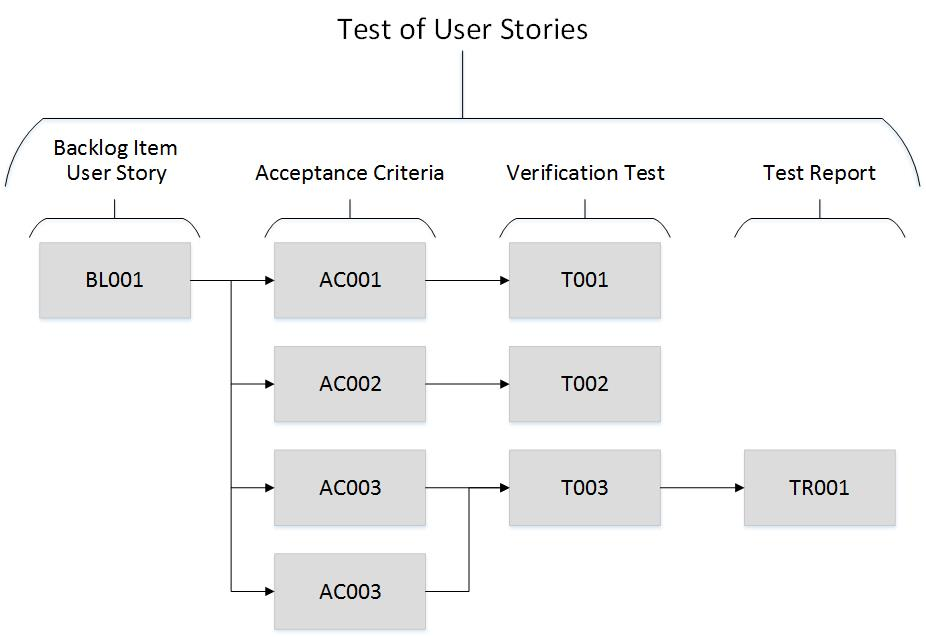
\includegraphics[width=0.9\textwidth]{VAPIQ-PICTURES/testdocbild}
        \caption{Test of User Stories}
        \label{fig:testsetup}
\end{figure}




